%% ----------------------------------------------------------------------------
% BIWI SA/MA thesis template
%
% Created 09/29/2006 by Andreas Ess
% Extended 13/02/2009 by Jan Lesniak - jlesniak@vision.ee.ethz.ch
%% ----------------------------------------------------------------------------
\newpage
\chapter{Related Work}

Describe the other's work in the field, with the following purposes in mind:

\begin{itemize}
    \item \textit{Is the overview concise?} Give an overview of the most relevant work to the needed extent. Make sure the reader can understand your work without referring to other literature.
    \item \textit{Does the compilation of work help to define the ``niche'' you are working in?} Another purpose of this section is to lay the groundwork for showing that you did significant work. The selection and presentation of the related work should enable you to name the implications, differences and similarities sufficiently in the ``discussion'' section.
\end{itemize}

\section{Diffusion Models}
\subsection{Forward Diffusion Process}

\begin{equation}
    \begin{split}
        q(x_t\mid x_{t-1}) & = \mathcal{N}(\sqrt{1-\beta_t} x_{t-1}, \beta_t I) \\
        q(x_t\mid x_{t-1}) & = \mathcal{N}(\sqrt{\alpha_t} x_{t-1}, (1-\alpha_t) I) \\
        q(x_t\mid x_{0}) & = \mathcal{N}(\sqrt{\bar{\alpha}_t} x_{0}, (1 - \bar{\alpha}_t) I) \\
        \bar{\alpha}_t & = \prod_{i=0}^{t} \alpha_t
    \end{split}
\end{equation}

\begin{figure}[h]
    \centering
    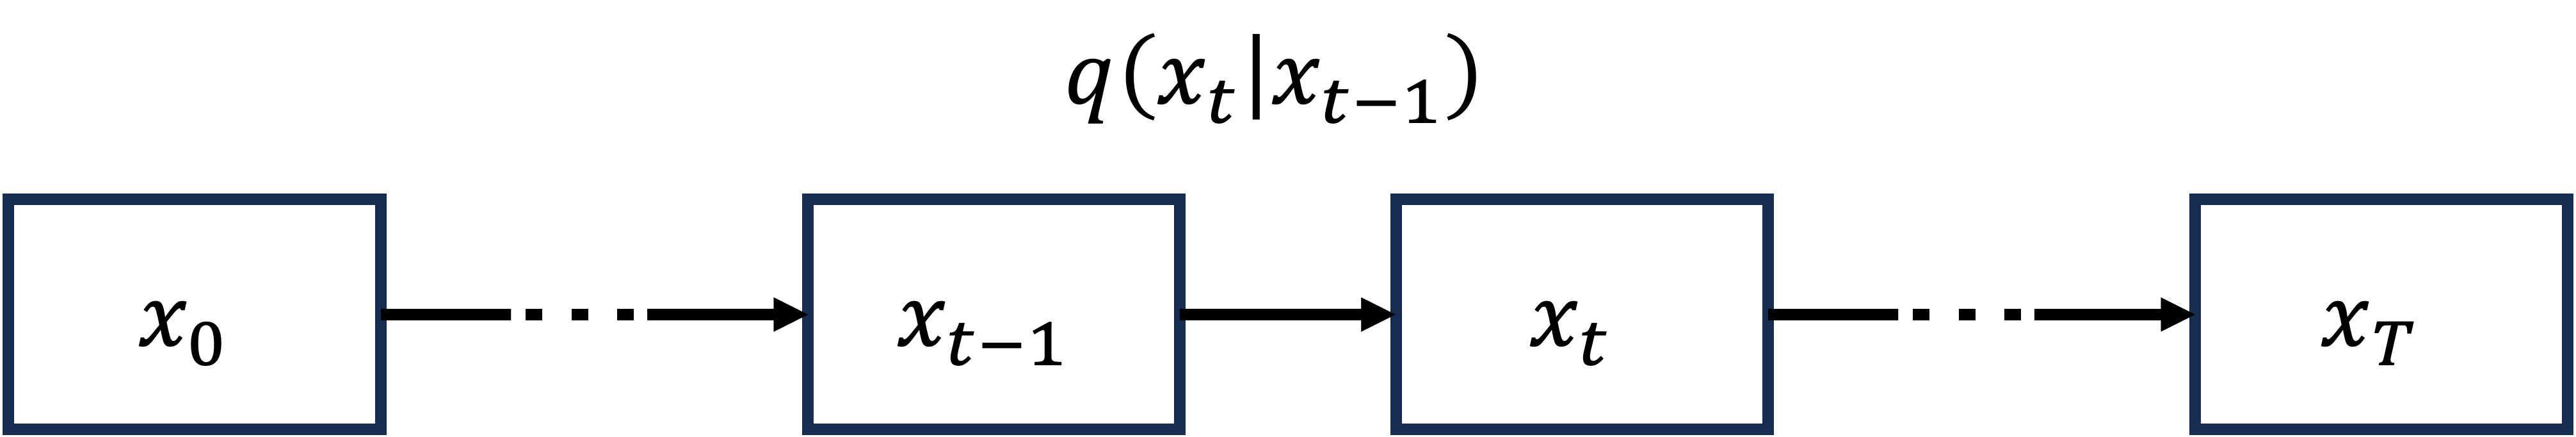
\includegraphics[width=.5\textwidth]{images/forward_diffusion.png}
    \caption{Forward Diffusion Process: An image is iteratively destroyed by adding normally distributed noise,
    according to a schedule. This represents a Markov process where the transition probability $q(x_t|x_{t-1})$.}
    \label{fig:forward_diffusion}
\end{figure}

\begin{figure}
    \centering
    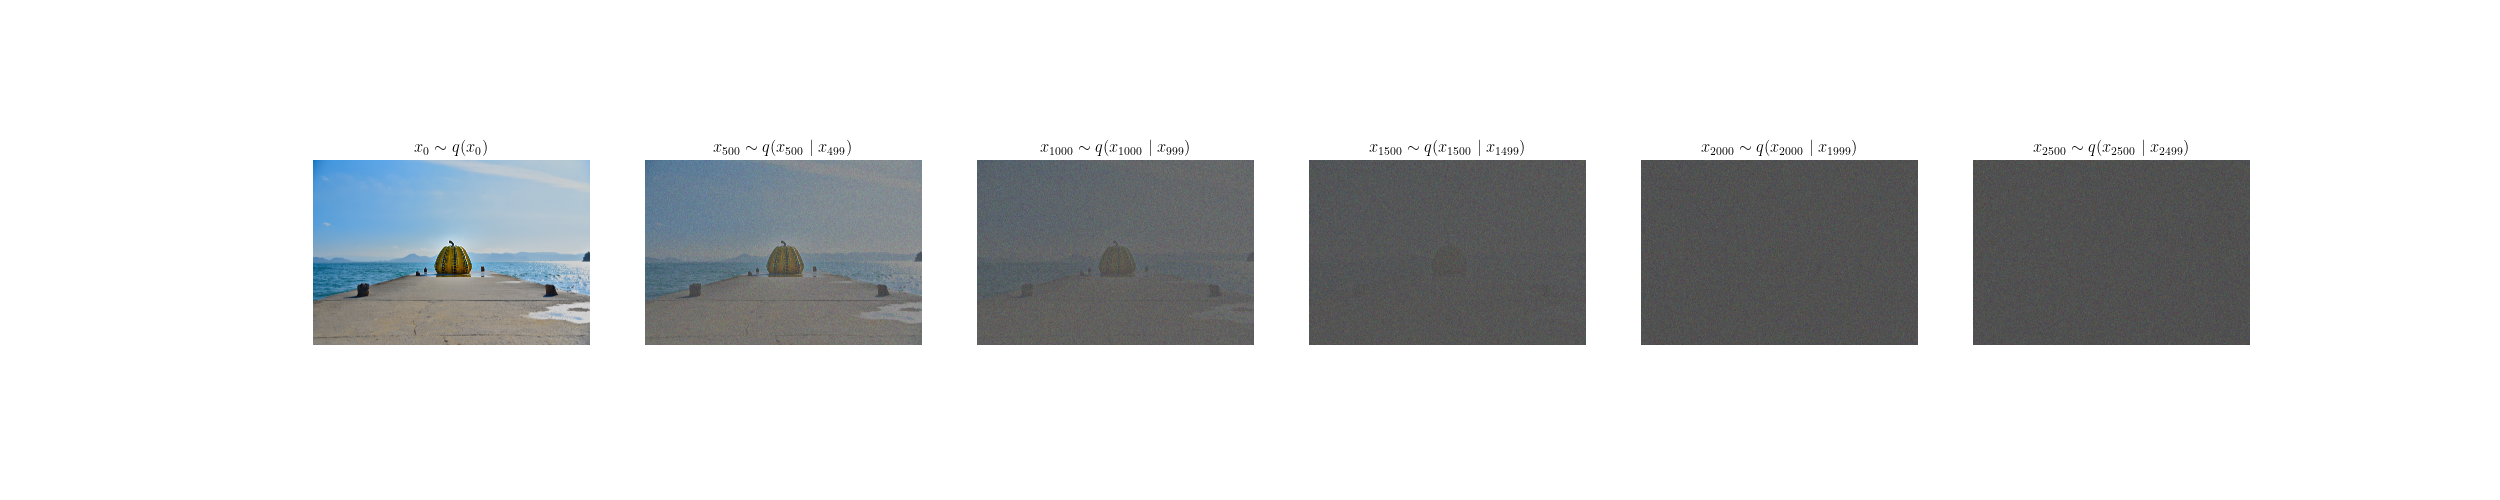
\includegraphics[width=\textwidth]{images/forward_naoshima.png}
    \caption{Example of Iterative Image Destruction through Forward Diffusion Process:
        The indices give the time step in the iterative destruction process, where $\beta$ was created according to a linear noise variance schedule (5000 steps from in the 0.001 to 0.02 range and picture resolution of 4016 by 6016 pixels).}
\end{figure}

\section{Excursion to Bayes}
Before getting started we need to quickly define the terms used in the next section, since they all stem from Bayesian
statistics. The Bayesian theorem can be written like this:
\begin{equation}
    p(z|x) = \frac{p(x|z)p(z)}{p(x)}
\end{equation}
It is implicitly assumed here that $p$ is a probability density function over two continuous random variables $x$ and $z$.
The formula holds in general, but in generative machine learning we usually assume that $z$ represents a random variable in
latent space (unobserved) from which we will eventually sample to generate new samples, whereas $x$ is the random variable that
represents the training images (observed space).
Using above described ordering, the four terms in this formula use distinct names:
\begin{description}
    \item[$p(z|x)$] is called the \textit{posterior}
    \item[$p(x|z)$] is called the \textit{likelihood}, since it gives the literal likelihood of observing an example $x$ when
        choosing the latent space to be a specific $z$.
    \item[$p(z)$] is called the \textit{prior}, since it exposes information on $z$ before any conditioning.
    \item[$p(x)$] is called the \textit{evidence}, since it encompasses our actual observations.
\end{description}
One of the most straightforward examples of a generative model where we search for such a latent space representation of
our distribution over the training examples, is the Variational Autoencoder (VAE)~\autocite{kingma2022autoencoding}. The name of the VAE stems from the Autoencoder,
a network that tries to recreate its output through a bottleneck and thereby learning a compressed representation of the data.~\autocite{https://doi.org/10.1002/aic.690370209}
It bears similarity to other dimension reduction methods like Principal Component Analysis (PCA) and therefore was first published under the name
\textit{Nonlinear principal component analysis}. The \textit{variational} part in the VAE stems from the fact that it tries to reduce the data not into
an arbitrary low dimensional latent space, but into a latent parameterized distribution (usually i.i.d multivariate Gaussian). This distribution is sampled
in the forward pass (therefore \textit{variational}, since we use a stochastic layer) and reproducing the input is now not a feasible loss function, but
maximizing the likelihood is. Maximizing the likelihood $p(x|z)$ from above means that we want to tune the parameters of this latent distribution such that the produced
output is \enquote{likely} an example that could come from the original distribution. Training generative models such as a VAE or also a GAN is usually either done with \textit{Evidence Lower Bound} as the loss, or with an additional network and an \textit{adversarial loss}.~\autocite{goodfellow2014generative} Both examples will be further explained in the next sections.

\section{Loss Functions}
In generative machine learning we would want our model to learn the distribution that generated
out training examples. Often this distribution is conditioned on some description (e.g. text) or
on the corruption process in our case, where we use generative models to solve inverse problems.
Assuming our original data distribution (of images) is $p(x)$, then we try to find a parameterized
variational machine learning model ($q_{\theta}(x)$) that will closely match the data distribution.

In order for this $q_{\theta}(x)$ to be trained we need a differentiable loss function that expresses
\enquote{closeness} in a distributional sense. The usual approach to this is to use the Kullback-Leibler (KL)
divergence.

\subsection{Kullback-Leibler Divergence}

\subsection{Wasserstein Distance}
A different approach to comparing the similarity of distributions is the Wasserstein metric, successfully used in the Wasserstein GAN.~\autocite{arjovsky2017wasserstein}.